% Report identifiers
% They are unique alphanumeric designations that may identify the responsible
% organization, the report series/collection and the individual report (i.e.
% Rapporti ISTISAN 05/2 stands for a report of the series Rapporti ISTISAN
% produced in the year 2005 and it is the second report of the year).

% ISSN/ISBN and other codes
% ISSN is the International Standard Serial Number that is assigned on request
% by the ISSN Authority (www.issn.org) for reports that are produced in a
% series; the ISBN is the International Standard Book Number that is assigned
% on request by the ISBN Authority to each single issue (www.isbn.org). The
% report may also have other codes, such as DOI (Digital Object Identifier),
% which may be obtained on request by each authority. More than one code may
% appear in a report.

% Place and date of publication
% It is important to include the place and date of publication, both for
% bibliographic identification and priority concerns. This information may
% appear in the title page or in the back of the title page.

% This document has been modified from its original version by Kathryn Huff
% Acknowledgement of the original version is below.
%
%%%%%%%%%%%%%%%%%%%%%%%%%%%%%%%%%%%%%%%%%
% Academic Title Page
% LaTeX Template
% Version 2.0 (17/7/17)
%
% This template was downloaded from:
% http://www.LaTeXTemplates.com
%
% Original author:
% WikiBooks (LaTeX - Title Creation) with modifications by:
% Vel (vel@latextemplates.com)
%
% License:
% CC BY-NC-SA 3.0 (http://creativecommons.org/licenses/by-nc-sa/3.0/)
%
% Instructions for using this template:
% This title page is capable of being compiled as is. This is not useful for
% including it in another document. To do this, you have two options:
%
% 1) Copy/paste everything between \begin{document} and \end{document}
% starting at \begin{titlepage} and paste this into another LaTeX file where you
% want your title page.
% OR
% 2) Remove everything outside the \begin{titlepage} and \end{titlepage}, rename
% this file and move it to the same directory as the LaTeX file you wish to add it to.
% Then add \input{./<new filename>.tex} to your LaTeX file where you want your
% title page.
%
%%%%%%%%%%%%%%%%%%%%%%%%%%%%%%%%%%%%%%%%%

%----------------------------------------------------------------------------------------
%    PACKAGES AND OTHER DOCUMENT CONFIGURATIONS
%----------------------------------------------------------------------------------------

\documentclass[11pt]{article}
\usepackage{draftwatermark}
\SetWatermarkText{DRAFT}
\SetWatermarkScale{1.2}
\SetWatermarkColor[gray]{0.95}
\usepackage[table]{xcolor}
\usepackage{tabularx}

\usepackage[utf8]{inputenc} % Required for inputting international characters
\usepackage[T1]{fontenc} % Output font encoding for international characters

\usepackage{mathpazo} % Palatino font
\usepackage{float}
\usepackage{graphicx,wrapfig} % For the logo and figures
\graphicspath{{./img/}}

% hyperref usually has to go last
\usepackage[hidelinks]{hyperref}
% but glossaries behaves best if after hyperref
\usepackage[acronym,toc]{glossaries}

% Allows for FloatBarrier
\usepackage{placeins}

\usepackage[colorinlistoftodos]{todonotes}
%\newacronym{<++>}{<++>}{<++>}
\newacronym[longplural={metric tons of heavy metal}]{MTHM}{MTHM}{metric ton of heavy metal}
\newacronym{ABM}{ABM}{agent-based modeling}
\newacronym{ACDIS}{ACDIS}{Program in Arms Control \& Domestic and International Security}
\newacronym{AHTR}{AHTR}{Advanced High Temperature Reactor}
\newacronym{ANDRA}{ANDRA}{Agence Nationale pour la gestion des D\'echets RAdioactifs, the French National Agency for Radioactive Waste Management}
\newacronym{ANL}{ANL}{Argonne National Laboratory}
\newacronym{API}{API}{application programming interface}
\newacronym{ARCH}{ARCH}{autoregressive conditional heteroskedastic}
\newacronym{ARE}{ARE}{Aircraft Reactor Experiment}
\newacronym{ARFC}{ARFC}{Advanced Reactors and Fuel Cycles}
\newacronym{ARMA}{ARMA}{autoregressive moving average}
\newacronym{ASME}{ASME}{American Society of Mechanical Engineers}
\newacronym{ATWS}{ATWS}{Anticipated Transient Without Scram}
\newacronym{BDBE}{BDBE}{Beyond Design Basis Event}
\newacronym{BIDS}{BIDS}{Berkeley Institute for Data Science}
\newacronym{BOL}{BOL}{Beginning-of-Life}
\newacronym{BSD}{BSD}{Berkeley Software Distribution}
\newacronym{CAFCA}{CAFCA}{ Code for Advanced Fuel Cycles Assessment }
\newacronym{CASL}{CASL}{Consortium for Advanced Simulation of Light Water Reactors}
\newacronym{CDTN}{CDTN}{Centro de Desenvolvimento da Tecnologia Nuclear}
\newacronym{CEA}{CEA}{Commissariat \`a l'\'Energie Atomique et aux \'Energies Alternatives}
\newacronym{CI}{CI}{continuous integration}
\newacronym{CNEC}{CNEC}{Consortium for Nonproliferation Enabling Capabilities}
\newacronym{CNEN}{CNEN}{Comiss\~{a}o Nacional de Energia Nuclear}
\newacronym{CNERG}{CNERG}{Computational Nuclear Engineering Research Group}
\newacronym{COSI}{COSI}{Commelini-Sicard}
\newacronym{COTS}{COTS}{commercial, off-the-shelf}
\newacronym{CSNF}{CSNF}{commercial spent nuclear fuel}
\newacronym{CTAH}{CTAHs}{Coiled Tube Air Heaters}
\newacronym{CUBIT}{CUBIT}{CUBIT Geometry and Mesh Generation Toolkit}
\newacronym{CURIE}{CURIE}{Centralized Used Fuel Resource for Information Exchange}
\newacronym{DAG}{DAG}{directed acyclic graph}
\newacronym{DANESS}{DANESS}{Dynamic Analysis of Nuclear Energy System Strategies}
\newacronym{DBE}{DBE}{Design Basis Event}
\newacronym{DESAE}{DESAE}{Dynamic Analysis of Nuclear Energy Systems Strategies}
\newacronym{DHS}{DHS}{Department of Homeland Security}
\newacronym{DOE}{DOE}{Department of Energy}
\newacronym{DRACS}{DRACS}{Direct Reactor Auxiliary Cooling System}
\newacronym{DRE}{DRE}{dynamic resource exchange}
\newacronym{DSNF}{DSNF}{DOE spent nuclear fuel}
\newacronym{DYMOND}{DYMOND}{Dynamic Model of Nuclear Development }
\newacronym{EBS}{EBS}{Engineered Barrier System}
\newacronym{EDZ}{EDZ}{Excavation Disturbed Zone}
\newacronym{EIA}{EIA}{U.S. Energy Information Administration}
\newacronym{EPA}{EPA}{Environmental Protection Agency}
\newacronym{EP}{EP}{Engineering Physics}
\newacronym{FCO}{FCO}{Fuel Cycle Options}
\newacronym{FCT}{FCT}{Fuel Cycle Technology}
\newacronym{FCWMD}{FCWMD}{Fuel Cycle and Waste Management Division}
\newacronym{FEHM}{FEHM}{Finite Element Heat and Mass Transfer}
\newacronym{FEPs}{FEPs}{Features, Events, and Processes}
\newacronym{FHR}{FHR}{Fluoride-Salt-Cooled High-Temperature Reactor}
\newacronym{FLiBe}{FLiBe}{Fluoride-Lithium-Beryllium}
\newacronym{GCAM}{GCAM}{Global Change Assessment Model}
\newacronym{GDSE}{GDSE}{Generic Disposal System Environment}
\newacronym{GDSM}{GDSM}{Generic Disposal System Model}
\newacronym{GENIUSv1}{GENIUSv1}{Global Evaluation of Nuclear Infrastructure Utilization Scenarios, Version 1}
\newacronym{GENIUSv2}{GENIUSv2}{Global Evaluation of Nuclear Infrastructure Utilization Scenarios, Version 2}
\newacronym{GENIUS}{GENIUS}{Global Evaluation of Nuclear Infrastructure Utilization Scenarios}
\newacronym{GPAM}{GPAM}{Generic Performance Assessment Model}
\newacronym{GRSAC}{GRSAC}{Graphite Reactor Severe Accident Code}
\newacronym{GUI}{GUI}{graphical user interface}
\newacronym{HLW}{HLW}{high level waste}
\newacronym{HPC}{HPC}{high-performance computing}
\newacronym{HTC}{HTC}{high-throughput computing}
\newacronym{HTGR}{HTGR}{High Temperature Gas-Cooled Reactor}
\newacronym{IAEA}{IAEA}{International Atomic Energy Agency}
\newacronym{IEA}{IEA}{International Energy Agency}
\newacronym{IEMA}{IEMA}{Illinois Emergency Mangament Agency}
\newacronym{INL}{INL}{Idaho National Laboratory}
\newacronym{IPRR1}{IRP-R1}{Instituto de Pesquisas Radioativas Reator 1}
\newacronym{IRP}{IRP}{Integrated Research Project}
\newacronym{ISFSI}{ISFSI}{Independent Spent Fuel Storage Installation}
\newacronym{ISRG}{ISRG}{Independent Student Research Group}
\newacronym{JFNK}{JFNK}{Jacobian-Free Newton Krylov}
\newacronym{LANL}{LANL}{Los Alamos National Laboratory}
\newacronym{LBNL}{LBNL}{Lawrence Berkeley National Laboratory}
\newacronym{LCOE}{LCOE}{levelized cost of electricity}
\newacronym{LDRD}{LDRD}{laboratory directed research and development}
\newacronym{LFR}{LFR}{Lead-Cooled Fast Reactor}
\newacronym{LGPL}{LGPL}{Lesser GNU Public License}
\newacronym{LLNL}{LLNL}{Lawrence Livermore National Laboratory}
\newacronym{LMFBR}{LMFBR}{Liquid-Metal-cooled Fast Breeder Reactor}
\newacronym{LOFC}{LOFC}{Loss of Forced Cooling}
\newacronym{LOHS}{LOHS}{Loss of Heat Sink}
\newacronym{LOLA}{LOLA}{Loss of Large Area}
\newacronym{LP}{LP}{linear program}
\newacronym{LWR}{LWR}{Light Water Reactor}
\newacronym{MARKAL}{MARKAL}{MARKet and ALlocation}
\newacronym{MA}{MA}{minor actinide}
\newacronym{MCNP}{MCNP}{Monte Carlo N-Particle code}
\newacronym{MILP}{MILP}{mixed-integer linear program}
\newacronym{MIT}{MIT}{the Massachusetts Institute of Technology}
\newacronym{MOAB}{MOAB}{Mesh-Oriented datABase}
\newacronym{MOOSE}{MOOSE}{Multiphysics Object-Oriented Simulation Environment}
\newacronym{MOX}{MOX}{mixed oxide}
\newacronym{MSBR}{MSBR}{Molten Salt Breeder Reactor}
\newacronym{MSRE}{MSRE}{Molten Salt Reactor Experiment}
\newacronym{MSR}{MSR}{Molten Salt Reactor}
\newacronym{NAGRA}{NAGRA}{National Cooperative for the Disposal of Radioactive Waste}
\newacronym{NCSA}{NCSA}{National Center for Supercomputing Applications}
\newacronym{NCSU}{NCSU}{North Carolina State University}
\newacronym{NEAMS}{NEAMS}{Nuclear Engineering Advanced Modeling and Simulation}
\newacronym{NEI}{NEI}{the Nuclear Energy Institute}
\newacronym{NERC}{NERC}{North American Electric Reliability Corporation}
\newacronym{NEUP}{NEUP}{Nuclear Energy University Programs}
\newacronym{NFCSim}{NFCSim}{Nuclear Fuel Cycle Simulator}
\newacronym{NFC}{NFC}{Nuclear Fuel Cycle}
\newacronym{NGNP}{NGNP}{Next Generation Nuclear Plant}
\newacronym{NMWPC}{NMWPC}{Nuclear MW Per Capita}
\newacronym{NNSA}{NNSA}{National Nuclear Security Administration}
\newacronym{NPRE}{NPRE}{Department of Nuclear, Plasma, and Radiological Engineering}
\newacronym{NQA1}{NQA-1}{Nuclear Quality Assurance - 1}
\newacronym{NRC}{NRC}{Nuclear Regulatory Commission}
\newacronym{NREL}{NREL}{the National Renewable Energy Laboratory}
\newacronym{NSF}{NSF}{National Science Foundation}
\newacronym{NSSC}{NSSC}{Nuclear Science and Security Consortium}
\newacronym{NUWASTE}{NUWASTE}{Nuclear Waste Assessment System for Technical Evaluation}
\newacronym{NWF}{NWF}{Nuclear Waste Fund}
\newacronym{NWTRB}{NWTRB}{Nuclear Waste Technical Review Board}
\newacronym{OCRWM}{OCRWM}{Office of Civilian Radioactive Waste Management}
\newacronym{ORION}{ORION}{ORION}
\newacronym{ORNL}{ORNL}{Oak Ridge National Laboratory}
\newacronym{PARCS}{PARCS}{Purdue Advanced Reactor Core Simulator}
\newacronym{PBAHTR}{PB-AHTR}{Pebble Bed Advanced High Temperature Reactor}
\newacronym{PBFHR}{PB-FHR}{Pebble-Bed Fluoride-Salt-Cooled High-Temperature Reactor}
\newacronym{PEI}{PEI}{Peak Environmental Impact}
\newacronym{PH}{PRONGHORN}{PRONGHORN}
\newacronym{PI}{PI}{Principal Investigator}
\newacronym{PJM}{PJM}{Pennsylvania-New Jersey-Maryland}
\newacronym{PNNL}{PNNL}{Pacific Northwest National Laboratory}
\newacronym{PRKE}{PRKE}{Point Reactor Kinetics Equations}
\newacronym{PSPG}{PSPG}{Pressure-Stabilizing/Petrov-Galerkin}
\newacronym{PWAR}{PWAR}{Pratt and Whitney Aircraft Reactor}
\newacronym{PWR}{PWR}{Pressurized Water Reactor}
\newacronym{PyNE}{PyNE}{Python toolkit for Nuclear Engineering}
\newacronym{PyRK}{PyRK}{Python for Reactor Kinetics}
\newacronym{QA}{QA}{quality assurance}
\newacronym{RDD}{RD\&D}{Research Development and Demonstration}
\newacronym{RD}{R\&D}{Research and Development}
\newacronym{RELAP}{RELAP}{Reactor Excursion and Leak Analysis Program}
\newacronym{RIA}{RIA}{Reactivity Insertion Accident}
\newacronym{RIF}{RIF}{Region-Institution-Facility}
\newacronym{SAM}{SAM}{Simulation and Modeling}
\newacronym{SCF}{SCF}{Software Carpentry Foundation}
\newacronym{SFR}{SFR}{Sodium-Cooled Fast Reactor}
\newacronym{SINDAG}{SINDA{\textbackslash}G}{Systems Improved Numerical Differencing Analyzer $\backslash$ Gaski}
\newacronym{SKB}{SKB}{Svensk K\"{a}rnbr\"{a}nslehantering AB}
\newacronym{SNF}{SNF}{spent nuclear fuel}
\newacronym{SNL}{SNL}{Sandia National Laboratory}
\newacronym{SNM}{SNM}{Special Nuclear Material}
\newacronym{STC}{STC}{specific temperature change}
\newacronym{SUPG}{SUPG}{Streamline-Upwind/Petrov-Galerkin}
\newacronym{SWF}{SWF}{Separations and Waste Forms}
\newacronym{SWU}{SWU}{Separative Work Unit}
\newacronym{SandO}{S\&O}{Signatures and Observables}
\newacronym{THW}{THW}{The Hacker Within}
\newacronym{TRIGA}{TRIGA}{Training Research Isotope General Atomic}
\newacronym{TRISO}{TRISO}{Tristructural Isotropic}
\newacronym{TSM}{TSM}{Total System Model}
\newacronym{TSPA}{TSPA}{Total System Performance Assessment for the Yucca Mountain License Application}
\newacronym{UFD}{UFD}{Used Fuel Disposition}
\newacronym{UIUC}{UIUC}{the University of Illinois at Urbana-Champaign}
\newacronym{UML}{UML}{Unified Modeling Language}
\newacronym{UOX}{UOX}{uranium oxide}
\newacronym{UQ}{UQ}{uncertainty quantification}
\newacronym{US}{US}{United States}
\newacronym{UW}{UW}{University of Wisconsin}
\newacronym{VISION}{VISION}{the Verifiable Fuel Cycle Simulation Model}
\newacronym{VV}{V\&V}{verification and validation}
\newacronym{WIPP}{WIPP}{Waste Isolation Pilot Plant}
\newacronym{YMG}{YMG}{Young Members Group}
\newacronym{YMR}{YMR}{Yucca Mountain Repository Site}

\makeglossaries

\begin{document}

%----------------------------------------------------------------------------------------
%    TITLE PAGE
%----------------------------------------------------------------------------------------

\begin{titlepage} % Suppresses displaying the page number on the title page and the subsequent page counts as page 1
    \newcommand{\HRule}{\rule{\linewidth}{0.5mm}} % Defines a new command for horizontal lines, change thickness here

    \center % Centre everything on the page

    %------------------------------------------------
    %    Title
    %------------------------------------------------
    \HRule
    \vspace{0.2cm}
     \begin{minipage}{0.4\textwidth}
        
\includegraphics[width=\textwidth]{./img/arfc-logo.png}
        \end{minipage}%
        \begin{minipage}{0.6\textwidth}
        {\begin{flushright}\huge\bfseries Economic and Carbon Impacts of Potential Illinois Nuclear Plant Closures\end{flushright}}
        {\begin{flushright}\large\textit{The Cost of Closures}\end{flushright}}
        \end{minipage}

    \vspace{0.2cm}
    \HRule
    \vspace{0.5cm}

    %------------------------------------------------
    %    Author(s)
    %------------------------------------------------
       \begin{minipage}{0.45\textwidth}
               \begin{flushleft}
                       \large
                       \textit{Prepared for:}\\
                       \textsc{Nuclear Matters}%
                       \vspace{4mm}\\ %
                       \textit{Principal Investigators:}\\ %
                       Prof. Kathryn D. \textsc{Huff} % Supervisor's name
                       Dr. Madicken \textsc{Munk} % Supervisor's name
                \end{flushleft}
       \end{minipage}
       ~
       \begin{minipage}{0.45\textwidth}
               \begin{flushright}
                       \large
                       \textit{Prepared by:}\\
                       Samuel G. \textsc{Dotson}\\ %
                       Amanda M. \textsc{Bachmann}\\ %
                       Zo\"{e} R. \textsc{Richter}\\ %
                       Nataly R. \textsc{Panczyk}\\ %
                       Nathan S. \textsc{Ryan}\\ %
                       Anna C. \textsc{Balla}\\ %
                       Erin R. \textsc{Fanning}
               \end{flushright}
    \end{minipage}

    % If you don't want a supervisor, uncomment the two lines below and comment the code above
    %{\large\textit{Author}}\\
    %John \textsc{Smith} % Your name

    %------------------------------------------------
    %    Report Number
    %------------------------------------------------
    \vspace{.5cm}
    \textsc{\LARGE\bfseries UIUC-ARFC-2021-01} % Replace YYYY with the year, NN with report index
    \vspace{0.2cm}

    %------------------------------------------------
    %    Date
    %------------------------------------------------

    \vspace{0.5cm} % Position the date further down the remaining page
    {\large April 30, 2021} % January 1, 3000
    % Use the date of actual publication, change the \today to a set date if you want to be precise
    \vspace{0.5cm}

%------------------------------------------------
    %    Headings
    %------------------------------------------------

    \textsc{\LARGE Advanced Reactors and Fuel Cycles}\\[0.25cm] % Research Group

    \textsc{\large Dept. of Nuclear, Plasma, \& Radiological Engineering}\\% Department

    \textsc{\large University of Illiois at Urbana-Champaign}\\ % University



    %------------------------------------------------
    %    Logo
    %------------------------------------------------

    \vspace{0.5cm}
    
\includegraphics[width=0.8\textwidth]{./img/illinois.eps}\\[1cm] % Include a department/university logo - this will require the graphicx package

    %----------------------------------------------------------------------------------------

    %------------------------------------------------
    %   Funding
    %------------------------------------------------
    % For this section, either use \vfill to fill the space
    % or insert funding acknowledgement
    \textit{This research was performed using funding received from Nuclear
    Matters.}

\end{titlepage}
%----------------------------------------------------------------------------------------
%\pagebreak

\section{Summary}
On August 27, 2020, Exelon Generation announced planned premature closures of 
two Illinois nuclear plants (4 reactor units), which compete economically with 
fossil fueled plants within the \gls{PJM} interconnection \cite{larson_exelon_2020}. 
This report quantitatively explores how these closures would undermine economic 
and decarbonization goals in the state of Illinois, such as an aggressive 
target to achieve a zero carbon electric grid by 2030.

Previous energy systems research has shown that such clean energy goals cannot 
be reached if nuclear plants prematurely retire 
\cite{national_academies_of_sciences_engineering_and_medicine_2021_accelerating_2021,larson_net-zero_2020,davis_net-zero_2018}.  
In particular, the February 2021 National Academy of Sciences, Engineering, and 
Medicine consensus report, ``Accelerating Decarbonization of the U.S. Energy 
System,'' determined unequivocally that U.S. decarbonization will require keeping 
existing nuclear plants open 
\cite{national_academies_of_sciences_engineering_and_medicine_2021_accelerating_2021}. 
Consistent with that literature, our simulations indicate that decarbonization 
in Illinois will require not only maintenance but expansion of nuclear energy capacity. 
\textbf{The simulations in this report minimize future Illinois electric system 
cost in the context of potential policy constraints and demonstrate that:}

\begin{itemize}
        \item nuclear energy is necessary to reach Illinois' carbon reduction 
                goals;
        \item without existing nuclear power, reaching zero carbon would 
                require solar deployments to displace $10,000km^2$ of critical 
                Illinois 
                farmland;
        \item and deploying new advanced nuclear generation is the least expensive way to 
                allow Illinois farmland to remain farmland while reaching 
                zero-carbon by 2030.
  \end{itemize}

\textbf{These simulations also revealed many specific, complementary 
conclusions, such as:}
\begin{itemize}
        \item Keeping Illinois' existing nuclear plants open through 
                2050 avoids 25 million metric tons of life-cycle CO$_2$ 
                emissions and 600,000 metric tons of e-waste.
        \item Even if advanced nuclear deployments experienced 200\% capital 
                cost overruns, total system cost impacts would be negligible.
        \item Deploying advanced nuclear avoids approximately 900,000 metric 
                tons of e-waste. 
        \item Significant, possibly infeasible, grid-scale battery storage capacity 
                is required to meet any zero-carbon target with renewable 
                penetration.
\end{itemize}


\section{Introduction}
% Text from proposal follows
the Temoa framework (Tools for Energy 
Model Optimization and Analysis)\cite{temoa}. Temoa is an open-source framework for 
simulating and optimizing energy systems developed at North Carolina State 
University. With our \gls{UIUC} microgrid model in 
Temoa (Figure 1), we are able to determine the optimal energy generation mix 
for the \gls{UIUC} microgrid for various objective functions (minimize carbon, 
minimize cost, etc.) while meeting system constraints (zero carbon by 2050, 
practical deployment speeds, realistic improvements in storage technology 
capabilities, etc.). The UIUC microgrid model includes transportation as well 
as campus steam, electric, and chilled water demand and provides cross-decadal 
deployment solutions which optimize the scenario objective function.



Eleven (11) carbon free nuclear power reactors at 6 sites produce the majority of
electricity in Illinois and critically underpin its clean energy future. This
report quantitatively demonstrates the role nuclear energy must play in
minimizing cost while meeting Illinois’ carbon goals
through 2050. We have conducted techno-economic optimizations of
the Illinois energy system to establish optimal energy generation scenarios with and without the
at-risk plants. With these, we compared and contrasted the economic and carbon implications of
these energy futures. In addition to emissions, this report also considers
other environmental impacts of available energy choices, such as land use and
waste burdens.

Two reactors at the Byron Generating Station together generate over 2 GWe of
emissions-free nuclear energy. This plant provides the Byron, Illinois region
with hundreds of skilled jobs and \$38 million annually in taxes.


% from sam's paper
Baker et. al found that increasing penetration of renewables increases grid 
volatility which exponentially increased the \gls{LCOE} of the energy system when 
subject to a mismatch penalty. They also found that energy storage becomes 
increas- ingly valuable for grid stability at or above 20\% renewable 
penetration.

\begin{table}[ht]
        \centering
        \begin{tabular}{lcccc}
                \hline
                \textbf{ID} & \textbf{Byron}      & \textbf{Other}  & \textbf{Zero} & \textbf{Renewable} \\
                            & \textbf{\& Dresden} & \textbf{Nuclear} & \textbf{Carbon} & \textbf{Growth}\\
                            & \textbf{Closures} & \textbf{Closures} &  \textbf{Target}  & \textbf{Rate}\\
                \hline
                        BAU1 & 
                        \cellcolor{red!25}premature & 
                        \cellcolor{orange!25}scheduled & 
                        \cellcolor{red!25}none &
                        \cellcolor{red!25}limited \\ 
                        BAU2 & 
                        \cellcolor{orange!25}scheduled & 
                        \cellcolor{orange!25}scheduled & 
                        \cellcolor{red!25}none &
                        \cellcolor{red!25}limited \\ 
                        BAU3 & 
                        \cellcolor{green!25}none & 
                        \cellcolor{green!25}none & 
                        \cellcolor{red!25}none &
                        \cellcolor{red!25}limited \\ 
                        CC1 & 
                        \cellcolor{red!25}premature & 
                        \cellcolor{orange!25}scheduled & 
                        \cellcolor{green!25}2030 &
                        \cellcolor{green!25}optimistic\\ 
                        CC2 & 
                        \cellcolor{orange!25}scheduled & 
                        \cellcolor{orange!25}scheduled & 
                        \cellcolor{green!25}2030 &
                        \cellcolor{green!25}optimistic\\ 
                        CC3 & 
                        \cellcolor{green!25}none & 
                        \cellcolor{green!25}none & 
                        \cellcolor{green!25}2030 &
                        \cellcolor{green!25}optimistic\\ 
                        XN1 & 
                        \cellcolor{red!25}premature & 
                        \cellcolor{orange!25}scheduled & 
                        \cellcolor{green!25}2030 &
                        \cellcolor{green!25}optimistic\\ 
                        XN2 & 
                        \cellcolor{orange!25}scheduled & 
                        \cellcolor{orange!25}scheduled & 
                        \cellcolor{green!25}2030 &
                        \cellcolor{green!25}optimistic\\ 
                        XN3 & 
                        \cellcolor{green!25}none & 
                        \cellcolor{green!25}none & 
                        \cellcolor{green!25}2030 &
                        \cellcolor{green!25}optimistic\\ 
                        ZN1 & 
                        \cellcolor{red!25}premature & 
                        \cellcolor{orange!25}scheduled & 
                        \cellcolor{green!25}2030 &
                        \cellcolor{orange!25}unlimited\\ 
                        ZN2 & 
                        \cellcolor{orange!25}scheduled & 
                        \cellcolor{orange!25}scheduled & 
                        \cellcolor{green!25}2030 &
                        \cellcolor{orange!25}unlimited\\ 
                        ZN3 & 
                        \cellcolor{green!25}none & 
                        \cellcolor{green!25}none & 
                        \cellcolor{green!25}2030 &
                        \cellcolor{orange!25}unlimited\\ 
                        \hline
        \end{tabular}
        \caption{A summary of the scenarios simulated in this work, 
        differentiated by their primary constraints.}
        \label{tab:scenarios}
\end{table}


\section{Methods}\label{sec:methods}
%describe the methods, the data, the assumptions, the scenarios, a brief few 
%sentences on Temoa itself.
This work collected data from multiple sources to populate a model of the 
Illinois electric grid, including existing generation capacities, potential 
generation technologies, the costs and wastes associated with each, and the 
electricity demand profile. This simulated representation of the state of 
Illinois relies on the Temoa framework, an open source tool built by 
researchers at \gls{NCSU}, which enables energy system optimization and 
techno-economic analysis 
\cite{decarolis_temoa_2010,decarolis_modelling_2016,decarolis_formalizing_2017}.

\subsection{Optimization Analysis}
This work established optimal solutions to 
various scenarios which illuminate the potential impact of nuclear plant 
closures and other policy options on the cost of power in Illinois. These 
simulations  also explore the state of Illinois' ability to meet its aggressive 
carbon goals with and without maintenance and expansion of nuclear power 
capacity. 

Assumptions and constraints in these simulated scenarios differentiate them. 
Each optimized scenario is the solution to a linear programming 
problem  comprised of two key components. First, the objective function in this 
case minimizes the total system cost of the energy grid in the state of 
Illinois. 
Such an objective function is stated thus:

\begin{align}
\intertext{minimize} 
        &\sum_{g=1}^G\int_{t=2030}^{t=2050} (c_g(t)x_g(t))\\
\intertext{where}
        G&=\text{number of generation technologies}&\nonumber\\
        x_g(t)&=\text{capacity of technology g in year t }[TW] &\nonumber\\
        c_g(t)&=\text{total cost of technology g in year t }\left[\frac{\$}{TW}\right]&\nonumber\\
              &= (l_g(t) + f_g(t) + v_g(t)cf_g(t)t)x_g(t)\nonumber\\
        l_g(t)&=\text{loan cost of technology g in year t }\left[\frac{\$}{TW}\right]&\nonumber\\
        f_g(t)&=\text{fixed cost of technology g in year t }\left[\frac{\$}{TW}\right]&\nonumber\\
        v_g(t)&=\text{variable cost of technology g in year t }\left[\frac{\$}{TWh}\right]&\nonumber\\
        cf_g(t)&=\text{capacity factor of technology g in year t }[\%] .&\nonumber
\end{align}

Second, a set of constraints limit the model solutions. In this case, such 
constraints include balancing electric supply with electric demand, reducing 
carbon to zero by 2030, specifying renewable energy and energy
storage deployment speeds, and limiting land use based on availability.
All begin with the same initial condition. 
Then, optimization 
proceeds by varying all free parameters within the scope of the defined 
constraints in order to meet the objective. Ultimately the simulation solution 
gives the energy generation mix, $\vec{x_g}$, for the Illinois electric grid that minimizes system cost. 
In this case, Temoa varies the 
deployed ratio of generation technologies on the Illinois electric grid, within 
the constraints of various policies, to minimize cost. The simulations each 
begin in the year 2020 and proceed through 2050. The initial condition in 2020 
represents the current electricity generation mix in the state of Illinois 
.

\FloatBarrier
\subsection{Data}
% paragraph on data sources

This model of Illinois' electric generation in the 
Temoa framework
is populated by robust data from a variety of sources.
Data sources for this model included multiple national and regional 
databases. Primarily, this work relied on federal and international databases from the 
Energy Information Administration 
\cite{us_energy_information_administration_eia_preliminary_2021,energy_information_administration_state_2020,us_energy_information_administration_eia_electric_2021,us_energy_information_administration_eia_illinois_2020}, 
the U.S. Geological Survey \cite{hoen_united_2018}, 
International Energy Agency \cite{lorenczik_projected_2020}, 
the Nuclear Energy Agency \cite{crozat_full_2018}, 
the Nuclear Regulatory Commission 
\cite{united_states_nuclear_regulatory_commission_illinois_2020}, 
the Intergovernmental Panel on Climate Change 
\cite{intergovernmental_panel_on_climate_change_annex_2014,intergovernmental_panel_on_climate_change_climate_2014,intergovernmental_panel_on_climate_change_climate_2014-1,intergovernmental_panel_on_climate_change_climate_2014-2},
the Interstate Renewable Energy Council 
\cite{sherwood_us_2009,sherwood_us_2010,sherwood_us_2011,brown_solid_1996,sherwood_us_2012,sherwood_us_2013,sherwood_us_2014}, 
the Department of Energy's EERE and NE offices 
\cite{us_department_of_energy_capital_2016}, and the National Renewable Energy 
Laboratory 
\cite{nrel_national_renewable_energy_laboratory_2020_2020,sengupta_national_2018}.
Industry sources included the World Nuclear Association
\cite{world_nuclear_association_nuclear_2017}
, 
the Nuclear Energy Institute 
\cite{desai_nuclear_2018,desai_nuclear_2020,murphy_impacts_2019,tessum_air_2019},
Rockland Capital Generation \cite{rockland_capital_natural_2021},
Sargent \& Lundy \cite{sargent__lundy_capital_2020}, 
Lazard \cite{ray_lazards_2020},
and others 
\cite{the_solar_foundation_national_2020,solar_energy_industries_association_illinois_2020,rutovitz_calculating_2015}.


% paragraph on reproducibility and location of data/analysis
This work was conducted in the open under a BSD-3 open-source license by the 
Advanced Reactors and Fuel Cycles group at the University of Illinois. All 
data, models, and assumptions used in his work can all be found and explored at 
open source repository at 
\url{https://github.com/arfc/2021-04-nm-illinois}{github.com/arfc/2021-04-nm-illinois}.

\FloatBarrier
\subsection{Scenarios Simulated}\label{sec:simulations}

The scenarios we conducted are described in Table \ref{tab:scenarios}.
All share the same objective function, which seeks to minimize total system cost.
They are clustered in four major categories. First, the business-as-usual cases 
(BAU) assume no carbon limit, while the carbon constrained cases (CC) assume a zero 
carbon target in 2030. Comparing these two simulation categories reveals the 
potential impact of carbon limits and premature nuclear energy closure on 
the minimum achievable cost. These simulations make conservative assumptions 
about the cost and availability of advanced nuclear power. 

To explore the importance of these assumptions, two additional classes of 
simulations were explored. In the XN (expensive nuclear) cases, advanced 
nuclear reactors are assumed to be twice as expensive to build than the best 
conservative estimates. In the ZN (zero advanced nuclear) cases, advanced 
nuclear power is not available in time to contribute to carbon reductions in 
Illinois before 2050. These scenarios are summarized in Table 
\ref{tab:scenarios}. 

\begin{table}[ht]
        \centering
        \begin{tabular}{lcccc}
                \hline
                \textbf{ID} & \textbf{Byron}      & \textbf{Other}  & \textbf{Zero} & \textbf{Renewable} \\
                            & \textbf{\& Dresden} & \textbf{Nuclear} & \textbf{Carbon} & \textbf{Growth}\\
                            & \textbf{Closures} & \textbf{Closures} &  \textbf{Target}  & \textbf{Rate}\\
                \hline
                        BAU1 & 
                        \cellcolor{red!25}premature & 
                        \cellcolor{orange!25}scheduled & 
                        \cellcolor{red!25}none &
                        \cellcolor{red!25}limited \\ 
                        BAU2 & 
                        \cellcolor{orange!25}scheduled & 
                        \cellcolor{orange!25}scheduled & 
                        \cellcolor{red!25}none &
                        \cellcolor{red!25}limited \\ 
                        BAU3 & 
                        \cellcolor{green!25}none & 
                        \cellcolor{green!25}none & 
                        \cellcolor{red!25}none &
                        \cellcolor{red!25}limited \\ 
                        CC1 & 
                        \cellcolor{red!25}premature & 
                        \cellcolor{orange!25}scheduled & 
                        \cellcolor{green!25}2030 &
                        \cellcolor{green!25}optimistic\\ 
                        CC2 & 
                        \cellcolor{orange!25}scheduled & 
                        \cellcolor{orange!25}scheduled & 
                        \cellcolor{green!25}2030 &
                        \cellcolor{green!25}optimistic\\ 
                        CC3 & 
                        \cellcolor{green!25}none & 
                        \cellcolor{green!25}none & 
                        \cellcolor{green!25}2030 &
                        \cellcolor{green!25}optimistic\\ 
                        XN1 & 
                        \cellcolor{red!25}premature & 
                        \cellcolor{orange!25}scheduled & 
                        \cellcolor{green!25}2030 &
                        \cellcolor{green!25}optimistic\\ 
                        XN2 & 
                        \cellcolor{orange!25}scheduled & 
                        \cellcolor{orange!25}scheduled & 
                        \cellcolor{green!25}2030 &
                        \cellcolor{green!25}optimistic\\ 
                        XN3 & 
                        \cellcolor{green!25}none & 
                        \cellcolor{green!25}none & 
                        \cellcolor{green!25}2030 &
                        \cellcolor{green!25}optimistic\\ 
                        ZN1 & 
                        \cellcolor{red!25}premature & 
                        \cellcolor{orange!25}scheduled & 
                        \cellcolor{green!25}2030 &
                        \cellcolor{orange!25}unlimited\\ 
                        ZN2 & 
                        \cellcolor{orange!25}scheduled & 
                        \cellcolor{orange!25}scheduled & 
                        \cellcolor{green!25}2030 &
                        \cellcolor{orange!25}unlimited\\ 
                        ZN3 & 
                        \cellcolor{green!25}none & 
                        \cellcolor{green!25}none & 
                        \cellcolor{green!25}2030 &
                        \cellcolor{orange!25}unlimited\\ 
                        \hline
        \end{tabular}
        \caption{A summary of the scenarios simulated in this work, 
        differentiated by their primary constraints.}
        \label{tab:scenarios}
\end{table}


%\begin{figure}
%  \centering
%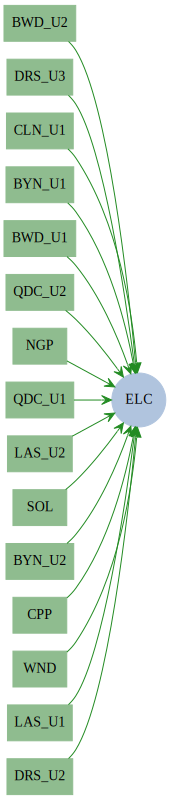
\includegraphics[width=0.3\linewidth]{../data/bau_illinois_input_graphviz/bau_illinois.png}
%\caption{The directed graph, implemented in Temoa, representing the electric grid in Illinois.} \label{fig:temoa_graph}
%\end{figure}



\FloatBarrier
\subsection{Constraints}
Some constraints are shared among all scenarios:
\begin{itemize}
        \item The initial conditions in 2020 reflect the true energy mix in Illinois in 2020.
        \item Power supply must meet power demand in each time step.
        \item Strategic planning reserve must be greater than 15\% of demand.
        \item Technology models are identical across all simulations with the exception of the capital cost of advanced nuclear, which is altered for the XN scenarios.  
\end{itemize}

The simulations diverge due to their differing treatment of constraints related 
to the timing of nuclear plant closures, inclusion of 
carbon targets, and land-use limits for the growth of renewables.

\subsubsection{Byron and Dresden Closures}
In each family of scenarios, the impact of closing Byron \& Dresden was explored 
by assuming one of three assumptions. The two plants either:
\begin{itemize} 
        \item close prematurely, in 2021,
        \item close as scheduled, when their current licenses expire in 20 and 10 
        years, or
        \item receive license extensions and continue operating through 2050.
\end{itemize}


\subsubsection{Other Existing Nuclear}
In each family of sencarios, the other existing nuclear power plants in 
Illinois were  either:
\begin{itemize}
        \item decommissioned as scheduled according to their current 
licenses, or 
        \item awarded license extensions and continue operating through 2050.
\end{itemize}

\subsubsection{Zero Carbon Target}
In the business as usual cases (BAU1-3), the simulations were not carbon limited. In all 
other simulations, a linear reduction in carbon emissions beginning in 2020 and 
reaching zero carbon emissions by 2030. This constrains energy 
deployment options in those simulations.

\subsubsection{Renewable Growth Rate}
In the business-as-usual cases, the growth rate for renewable energy is limited by economics, 
primarly. In the carbon constrained and expensive nuclear scenarios, an 
optimistic growth rate is enabled.
In those cases, utility scale solar is allowed to grow to 10 GWe by 2030, 
reflecting the aggressive and optimistic build out proposed in the Illinois 
Clean Energy Jobs Act. Similarly, wind turbine deployments grow to 13.8 GWe 
by 2030. Finally, residential solar is allowed to 
increase at a steady rate, but is capped at 75\% of the technical resource 
availability to reflect deployment on 75\% of Illinois buildings 
\cite{gagnon_rooftop_2016}. 

Without preserving existing nuclear or deploying advanced reactors, the
required land use for solar and wind generation is infeasible, since the 
Illinois land appropriate for wind and solar is already in use as vital 
farmland. The southern and central regions of Illinois most suitable for solar 
power installations are the same regions the nation currently relies on for 
15\% of its corn and 14\% of its soybeans \cite{schleusener_illinois_2020}.  

\begin{figure}[htbp!]
        \begin{center}
                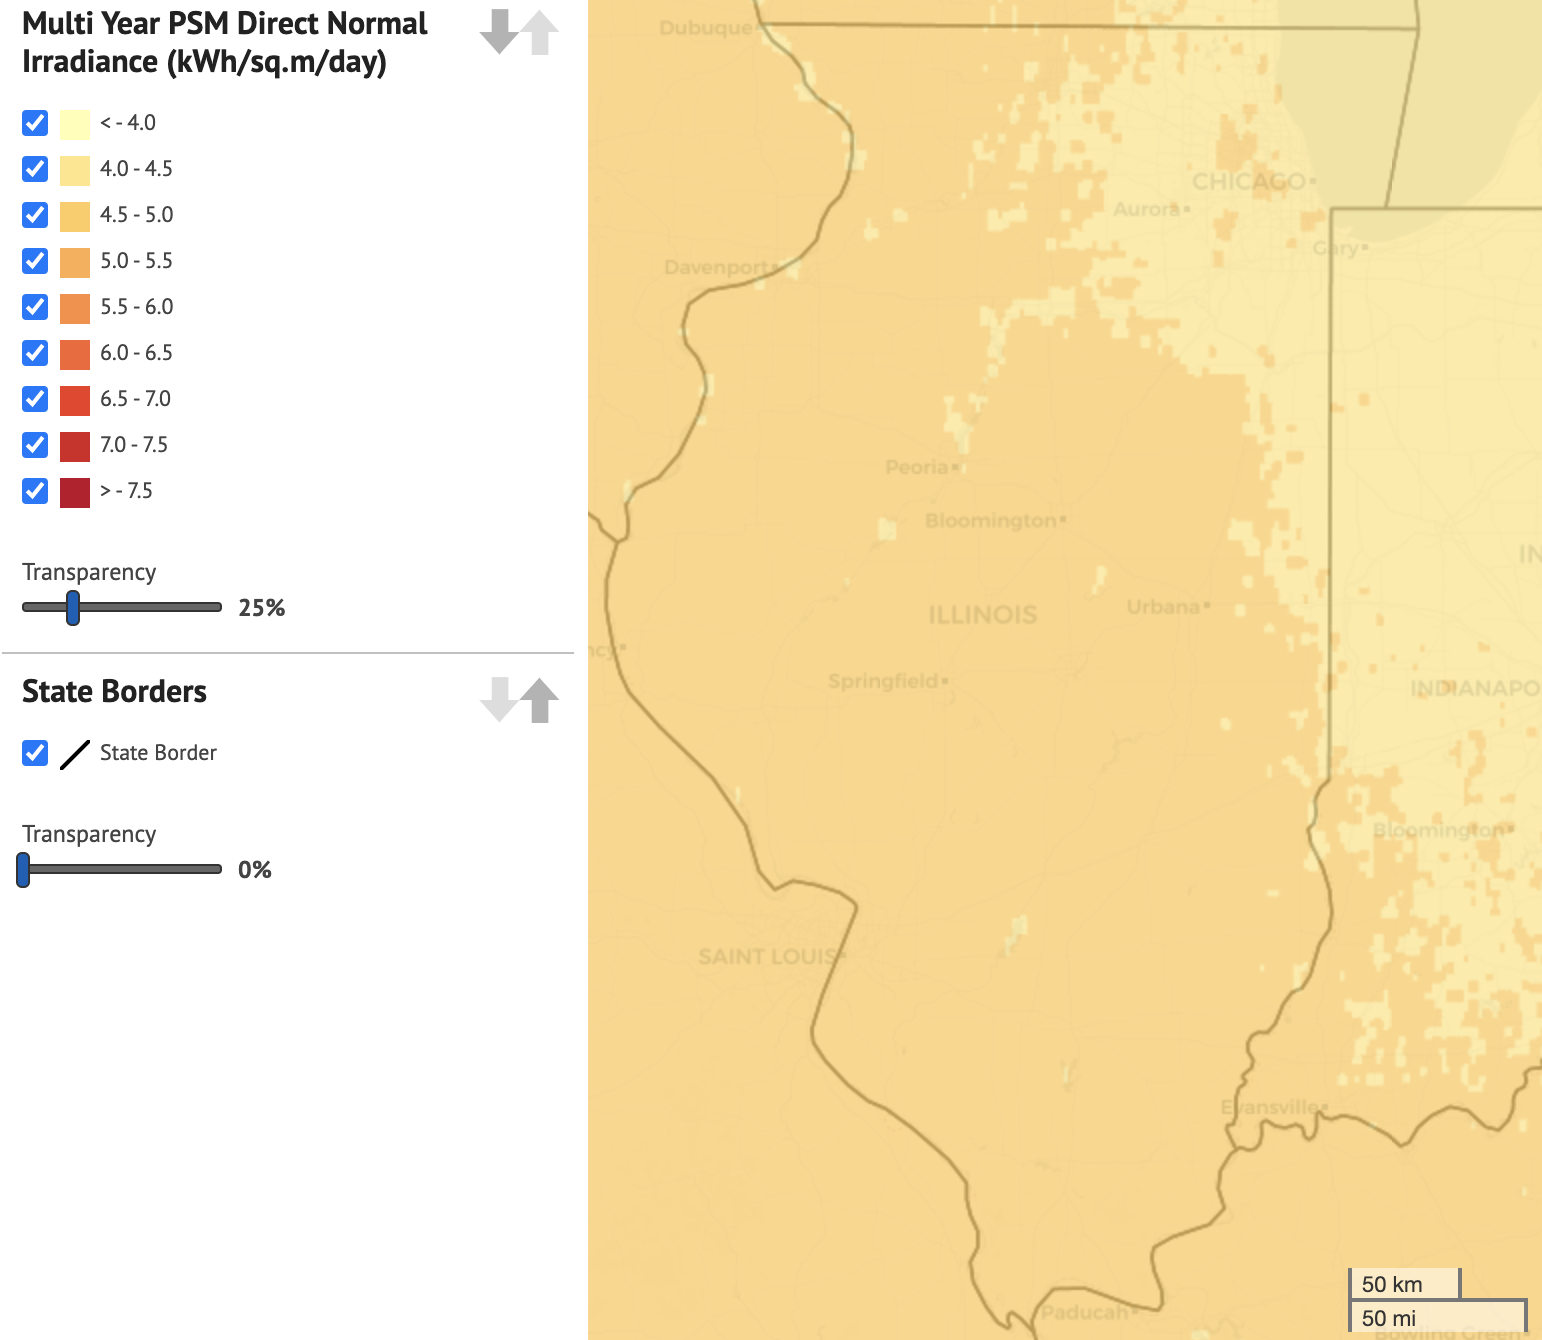
\includegraphics[height=0.4\textheight]{solar-suitability.png}\\
                \vspace{0.5cm}
                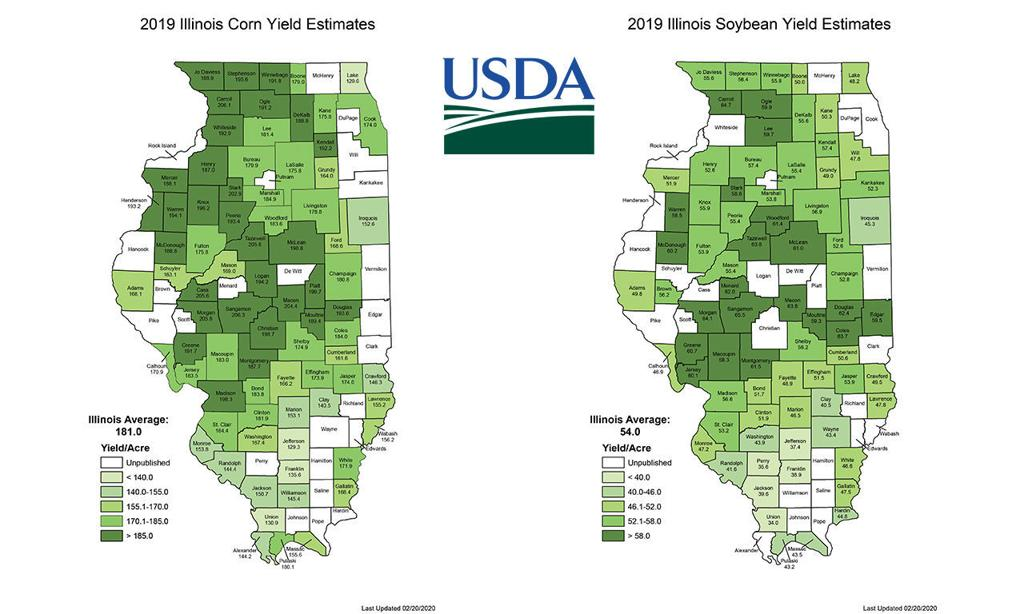
\includegraphics[width=\textwidth]{corn-and-soy.png}
        \end{center}
        \caption{Corn (bottom left) and soybean (bottom right) crops in Illinois lie predominantly in the 
        same portion of the state corresponding to the 
        region of highest solar panel suitability (top) 
        \cite{schleusener_illinois_2020,eispc_energy_2021,sengupta_national_2018}.}
        \label{fig:corn-and-soy}
\end{figure}


Specifically, strategies which allow nuclear plants to close before 2050 require 10,000$km^2$ of this land to be dedicated to solar as well as 4\% of Illinois' land area in use for rooftop solar. Keeping the nuclear plants open through 2050 halves this requirement.  
The constraints on utility scale wind and solar are lifted. It is not possible to achieve zero carbon without advanced nuclear under the above constraints.

\FloatBarrier
\subsection{Technology Models}
The technology models in Temoa representing energy source are configured with 
data regarding fundamental techno-economic parameters such as their capacity, 
capacity factors, seasonal generation profiles, auxilliary products, waste 
generation metrics, and costs (fixed, capital, variable, and otherwise). 
The following subsections describe the key assumptions about electricity 
generation and storage technologies in the Illinois model built for this 
report.

\subsubsection{Solar Energy Model}
Existing solar power capacities and cost data were averaged over the state and 
based on the \gls{NREL} Annual Technology Baseline for 2020. However, power 
generation profiles loaded into Temoa representing the variability of solar 
power, such as the seasonal variation in Figure 
\ref{fig:seasonal_hourly_solar}, were derived from a reference solar farm, UIUC Solar Farm 1.0, located in Champaign, IL. The data was provided by the University of Illinois Facilities and Services Department.
\FloatBarrier

\begin{figure}[H]
	\centering
	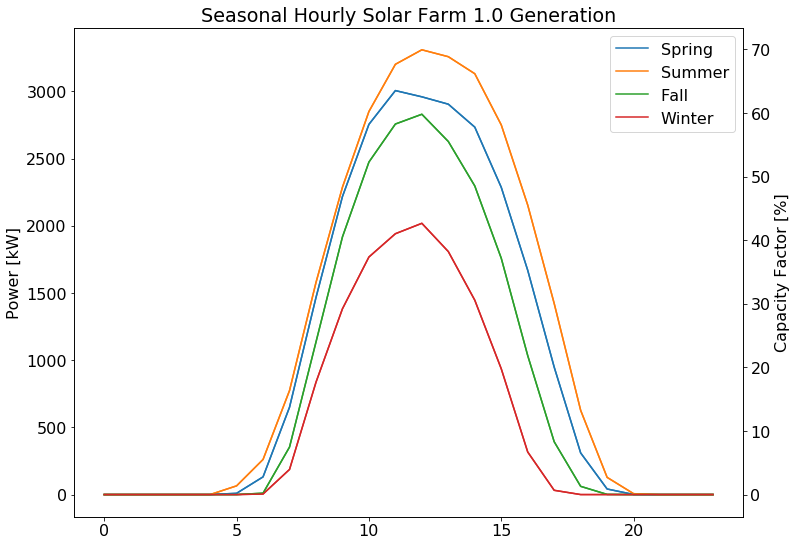
\includegraphics[width=0.7\columnwidth]{./img/seasonal_hourly_solar.png}
	\caption{}
	\caption{The seasonal variation in hourly generation from Solar Farm 
        1.0 at \gls{UIUC}, used as a scaled reference in the Temoa model of the Illinois grid. }
	\label{fig:seasonal_hourly_solar}
\end{figure}

\FloatBarrier

\subsubsection{Wind Energy Model}
Existing wind power capacities, capacity factors, and cost data were averaged over the state and 
based on the \gls{NREL} Annual Technology Baseline for 2020. However, power 
generation profiles loaded into Temoa representing the variability of wind 
generation, such as the seasonal variation in Figure 
\ref{fig:seasonal_hourly_wind}, were derived from a reference wind farm, Railsplitter Wind Farm, 
located in Lincoln, IL. The data was provided by the University of Illinois 
Facilities and Services Department. UIUC has a power purchase agreement with Railsplitter Wind 
Farm.


\begin{figure}[H]
	\centering
	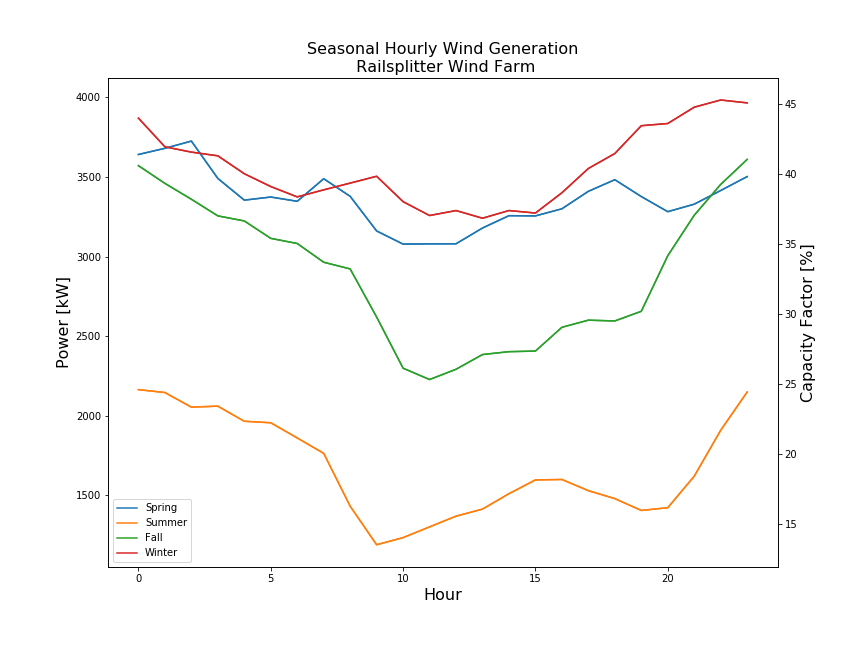
\includegraphics[width=0.7\columnwidth]{./img/cap/seasonal_hourly_wind.png}
	\caption{The seasonal variation in hourly generation from the Railsplitter Wind Farm, used as a scaled reference in the Temoa model of the Illinois grid. }
	\label{fig:seasonal_hourly_wind}
\end{figure}
\FloatBarrier

\subsubsection{Nuclear Energy Model}
Existing nuclear plants in Illinois were specified in the model in accordance with their 
power levels, licensed lifetimes, capacity factors, and costs. Advanced nuclear power plants, 
when available to the model, used pricing from the \gls{NREL} Annual Technology 
Baseline as well as the \gls{NEI} Nuclear Costs in Context report series
\cite{desai_nuclear_2020,desai_nuclear_2018}.

\subsubsection{Battery Technology}

Grid operators must plan for resource adequacy, and these simulations adopted the standard \gls{NERC} recommendation for planning reserve margin, defined as: 
\begin{align}
         PRM &= \frac{ C_{\text{firm}} - D_{\text{peak}} }{ D_{\text{peak}} }\\
        \intertext{where}
        C_{\text{firm}} &= \text{The firm capacity  [GW]}\nonumber\\
        D_{\text{peak}} &= \text{The peak demand  [GW]}.\nonumber
\end{align}

Firm capacity is sometimes considered the amount of power guaranteed to be
available for the duration of a commitment. We consider firm capacity to be the
amount of power that is available ``on-demand.'' Thus, renewable energy sources
do not contribute to firm capacity. In simulations requiring carbon free
electricity by 2030 in, the only technologies available to contribute to firm
capacity are nuclear power and battery storage. 

\subsubsection{Coal Energy Model}
Coal emissions (NO$_x$, SO$_x$, and CO$_2$) data were retrieved from the 2020 
Sargent and Lundy report, ``Capital Costs and Performance Characteristics for 
Utility Scale Power Generating Technologies'' \cite{sargent__lundy_capital_2020}.

\subsubsection{Natural Gas Energy Model}
Natural gas emissions (NO$_x$, SO$_x$, and CO$_2$) data were retrieved from the 
2020 Sargent and Lundy report on Capital Costs and Performance Characteristics 
for Utility Scale Power Generating Technologies 
\cite{sargent__lundy_capital_2020}.
\subsection{Demand Model}
Illinois electricity demand has remained steady at approximately 140.7 TWh per 
year for the last decade 
\cite{us_energy_information_administration_eia_illinois_2020}. All scenarios 
simulated in this report assume that this demand remains steady annually.
If Illinois transportation is fully electrified by 2050, this assumption will 
not be valid.  However, postulating such growth scenarios is  beyond the scope 
of this report. 

As part of model configuratino, the Temoa framework accepts demand profiles 
capturing seasonal and daily fluctuations. The typical Illinois hourly demand profile and seasonal variation in hourly demand were both retrieved from the \gls{EIA} 
\cite{us_energy_information_administration_eia_illinois_2020}. Figure 
\ref{fig:seasonal_hourly_demand} shows the variation in hourly demand.
In our simulations, the demand is seasonally modulated by this information.



\begin{figure}[htbp!]
        \begin{center}
               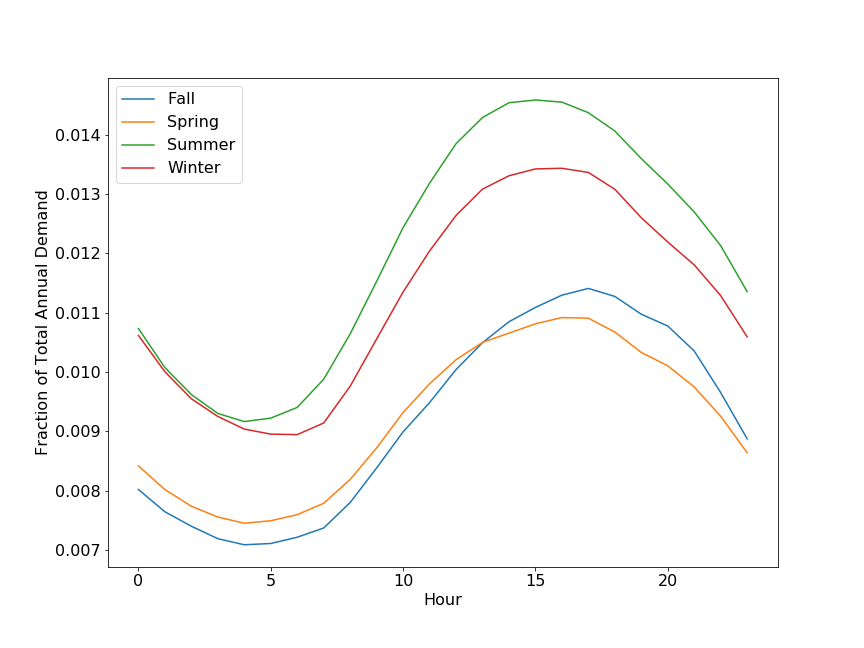
\includegraphics[width=0.8\textwidth]{seasonal_hourly_demand.png}
        \caption{The seasonal variation in hourly demand in Illinois was retrieved from the \gls{EIA} 
        \cite{us_energy_information_administration_eia_illinois_2020} and 
        loaded into Temoa \cite{decarolis_modelling_2016}.}
        \label{fig:seasonal_hourly_demand}
        \end{center}
\end{figure}

\subsection{Cost Modeling}
Where available price and cost data could only be found for previous years, we 
                accounted for the time value of money by adjusting for 
                inflation using the consumer price index from the 
                Bureau of Labor Statistics \cite{bls_consumer_2021}. The 
                adjusted price becomes: 

\begin{align}
        P_{2020} &= \mbox{adjusted price in 2020 dollars }[\$]\\
                &= \frac{P_{n} \cdot CPI_{2020}}{CPI_{n}}\\
        \intertext{where}
        P_n &= \mbox{price in year previous year, n } [\$]\\
        CPI_{2020} &= \mbox{consumer price index for 2020 } [-]\\
        CPI_n &= \mbox{consumer price indes for year n } [-].
\end{align}


\subsection{Carbon Pricing of Life Cycle Emissions}
All energy generation technologies have some life cycle emissions.
In order to account for the cost of lifecycle carbon emissions from each 
technology, a carbon price was applied to the fixed cost of renewables and 
nuclear, thus,

\begin{align}
P_c &= \left[\frac{\$}{tCO2}\right] = \left[\frac{M\$}{MTCO2}\right]\\
R_c &= \left[\frac{MTCO2}{GWh}\right]\\\\
FC_c &= R_c\cdot P_c \cdot CF \cdot \frac{hours}{year} = \left[\frac{M\$}{GW-year}\right]
\end{align}

For fossil fuels, this price was included in their variable costs.

\section{Results}
%describe the results, stick to the facts.






\begin{figure}[ht]
	\centering
	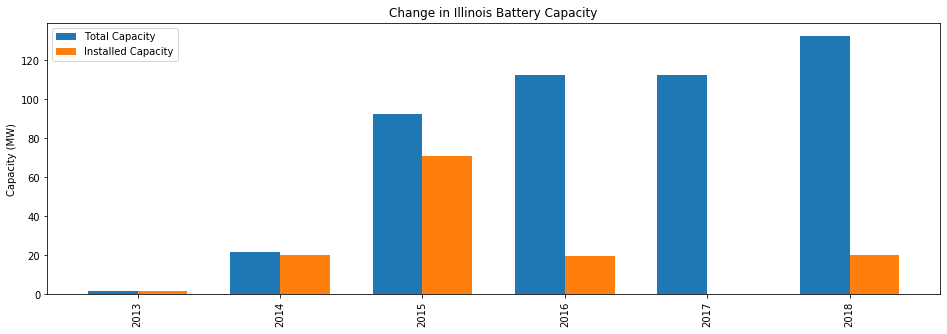
\includegraphics[width=\columnwidth]{./img/annual_installed_cap_battery.png}
	\caption{<++>}
	\label{fig:<++>}
\end{figure}


\begin{figure}[ht]
	\centering
	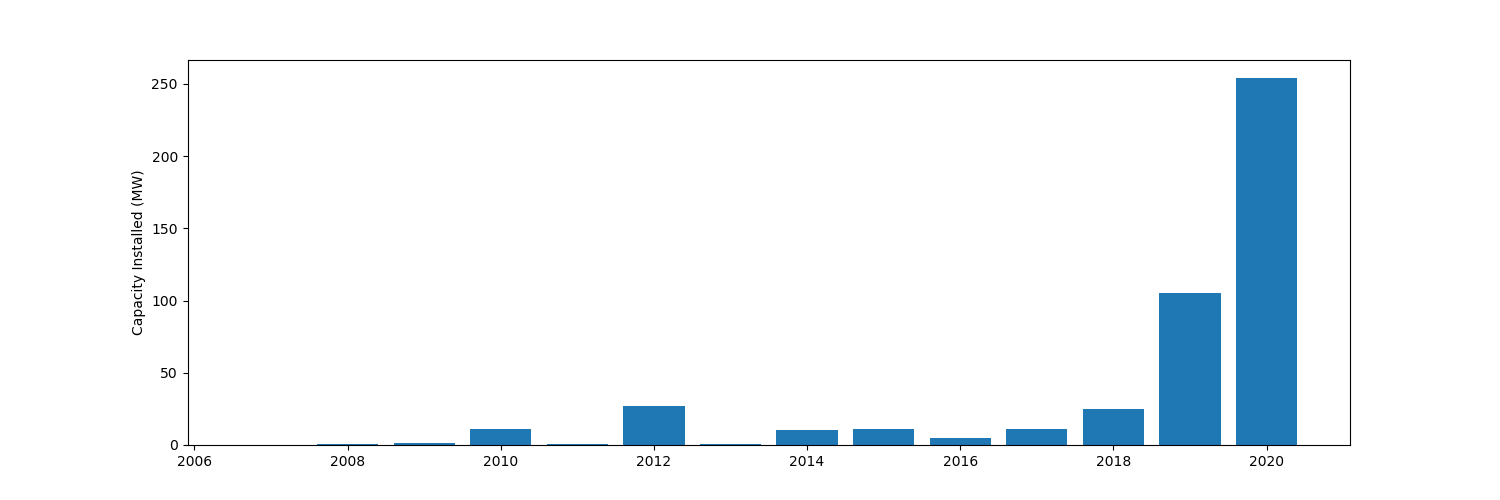
\includegraphics[width=\columnwidth]{./img/annual_installed_cap_solar.png}
	\caption{<++>}
	\label{fig:<++>}
\end{figure}


\begin{figure}[ht]
	\centering
	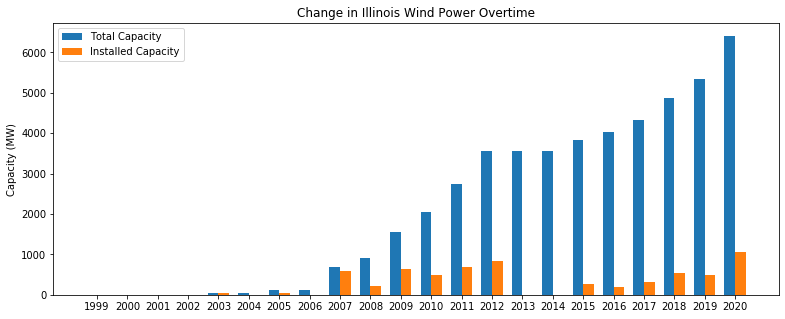
\includegraphics[width=\columnwidth]{./img/annual_installed_cap_wind.png}
	\caption{<++>}
	\label{fig:<++>}
\end{figure}


\begin{figure}[ht]
	\centering
	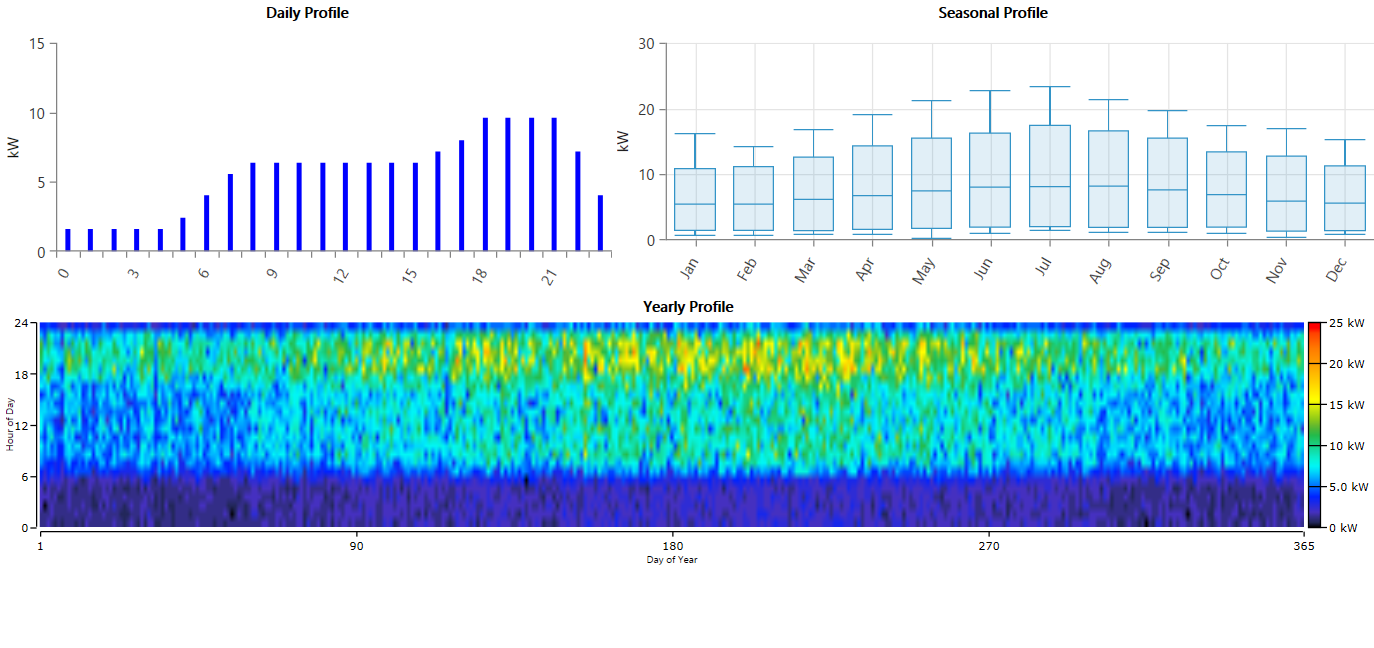
\includegraphics[width=\columnwidth]{./img/homer_illinois_loadprofile.png}
	\caption{<++>} 
        \label{fig:<++>}
\end{figure}


\begin{figure}[ht]
	\centering
	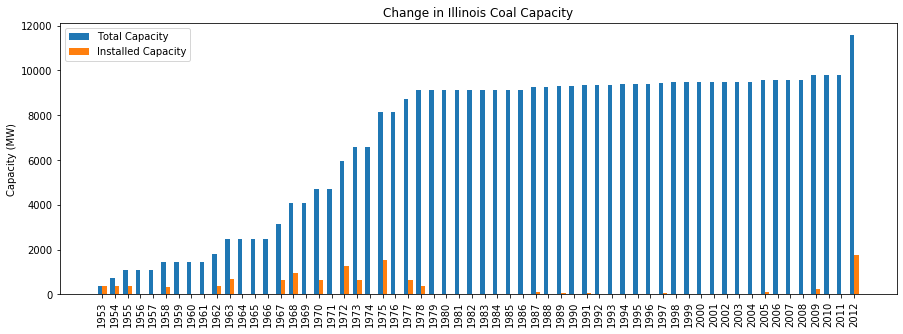
\includegraphics[width=\columnwidth]{./img/annual_installed_cap_coal.png}
	\caption{<++>}
	\label{fig:<++>}
\end{figure}


\begin{figure}[ht]
	\centering
	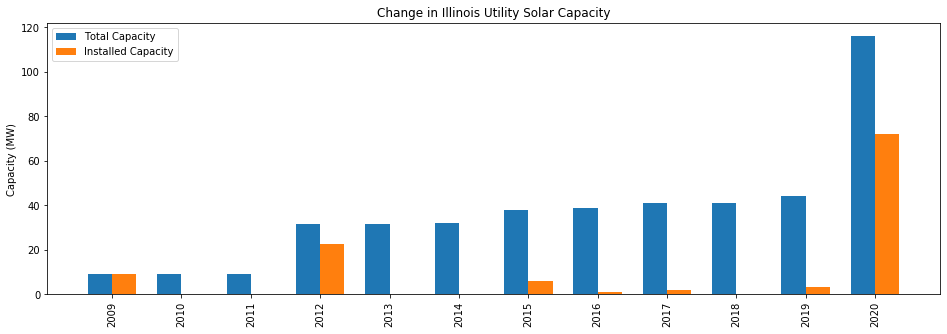
\includegraphics[width=\columnwidth]{./img/annual_installed_cap_utilityPV.png}
	\caption{<++>}
	\label{fig:<++>}
\end{figure}


\begin{figure}[ht]
	\centering
	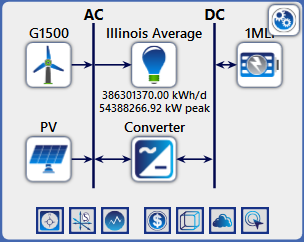
\includegraphics[width=\columnwidth]{./img/homer_system_setup.png}
	\caption{<++>}
	\label{fig:<++>}
\end{figure}


\begin{figure}[ht]
	\centering
	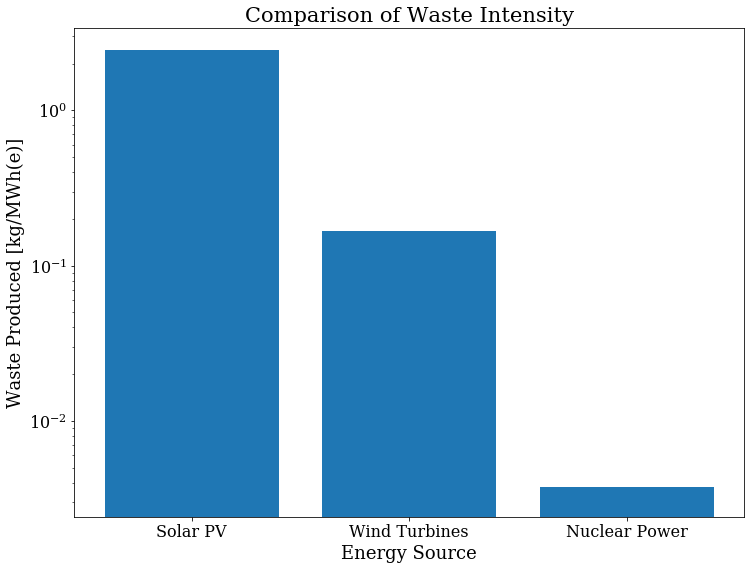
\includegraphics[width=\columnwidth]{./img/mass-waste-intensity.png}
	\caption{<++>}
	\label{fig:<++>}
\end{figure}


\begin{figure}[ht]
	\centering
	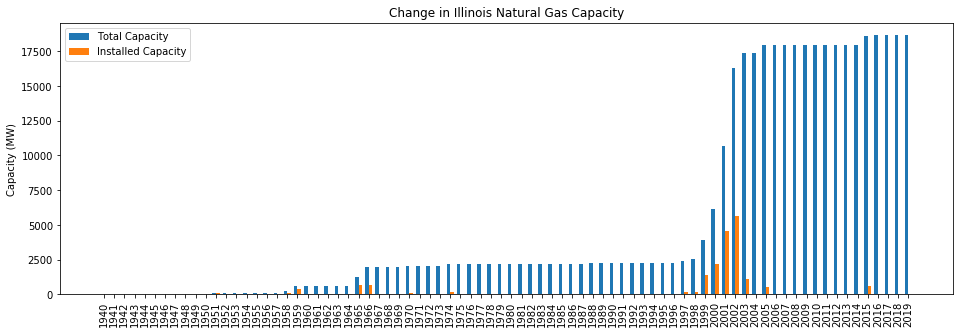
\includegraphics[width=\columnwidth]{./img/annual_installed_cap_natgas.png}
	\caption{<++>}
	\label{fig:<++>}
\end{figure}

\begin{figure}[ht]
	\centering
	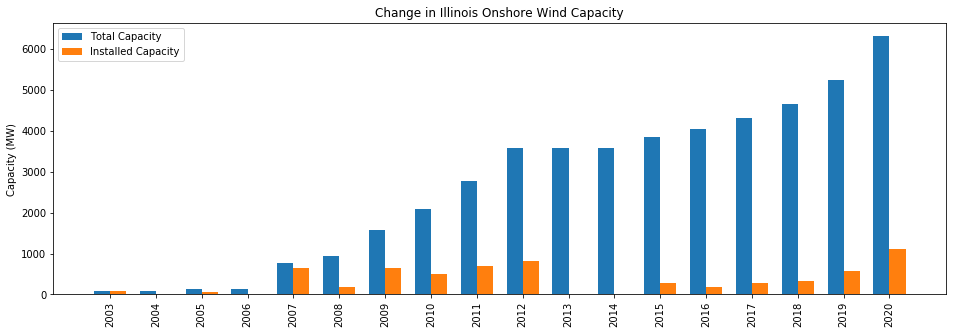
\includegraphics[width=\columnwidth]{./img/annual_installed_cap_utilitywind.png}
        \caption{<++>}
	\label{fig:<++>}
\end{figure}



\begin{figure}[ht]
	\centering
        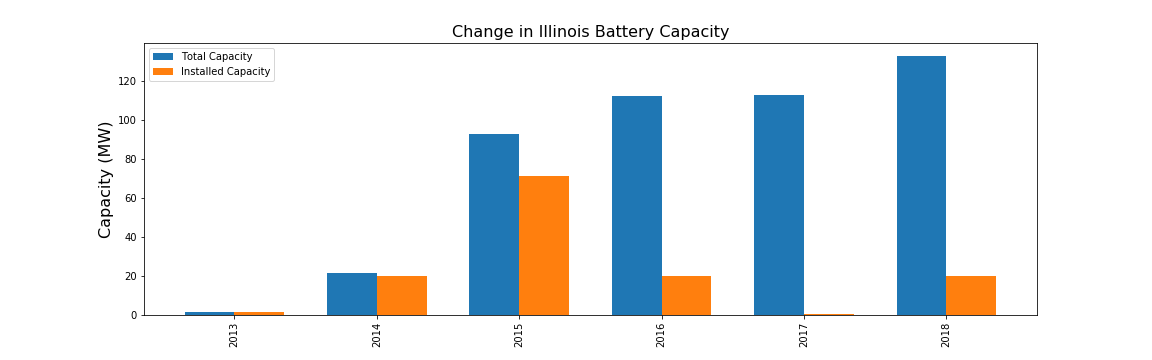
\includegraphics[width=\columnwidth]{./img/cap/battery.png}
	\caption{<++>}
	\label{fig:<++>}
\end{figure}

\begin{figure}[ht]
	\centering
	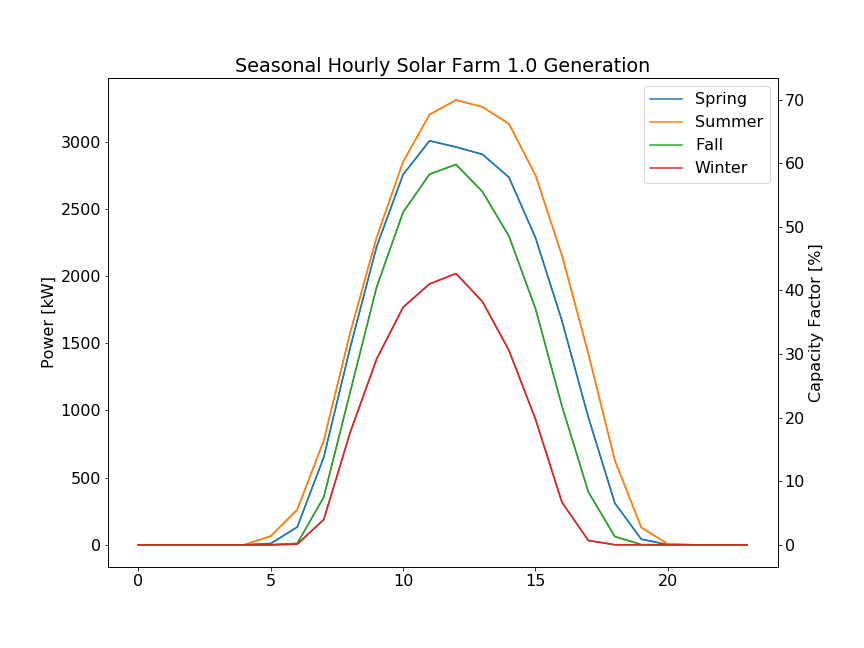
\includegraphics[width=\columnwidth]{./img/cap/seasonal_hourly_solar.png}
	\caption{<++>}
	\label{fig:<++>}
\end{figure}

\begin{figure}[ht]
	\centering
	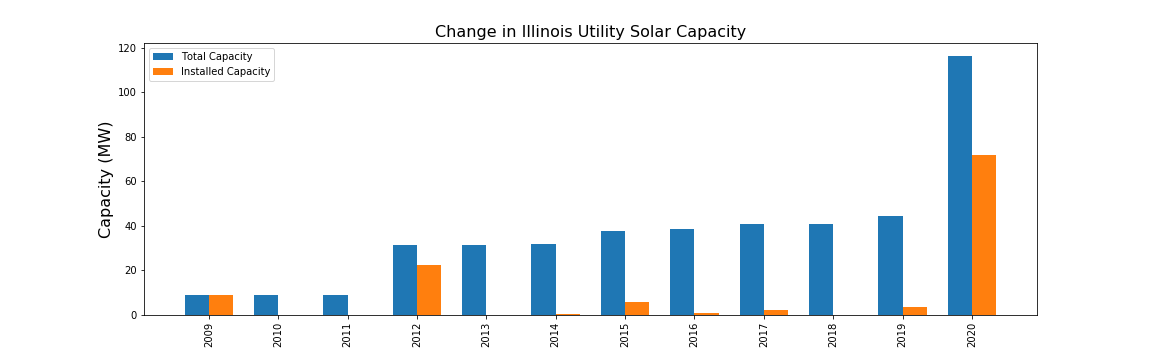
\includegraphics[width=\columnwidth]{./img/cap/solar.png}
	\caption{<++>}
	\label{fig:<++>}
\end{figure}

\begin{figure}[ht]
	\centering
	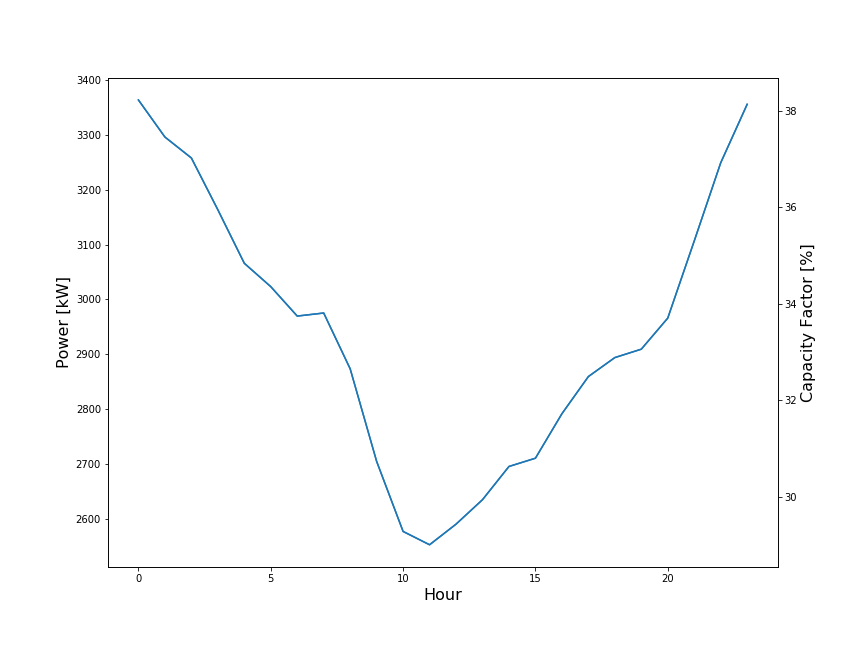
\includegraphics[width=\columnwidth]{./img/cap/wind_cf.png}
	\caption{<++>}
	\label{fig:<++>}
\end{figure}

\begin{figure}[ht]
	\centering
	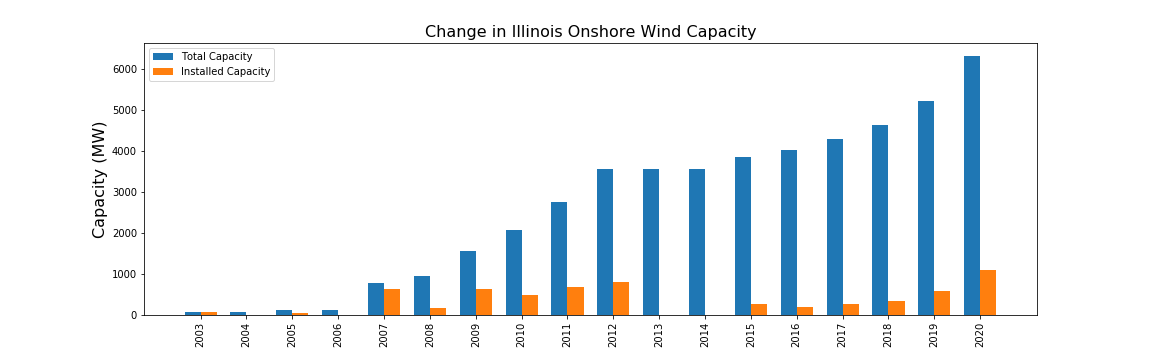
\includegraphics[width=\columnwidth]{./img/cap/onshore_wind.png}
	\caption{<++>}
	\label{fig:<++>}
\end{figure}

\begin{figure}[ht]
	\centering
	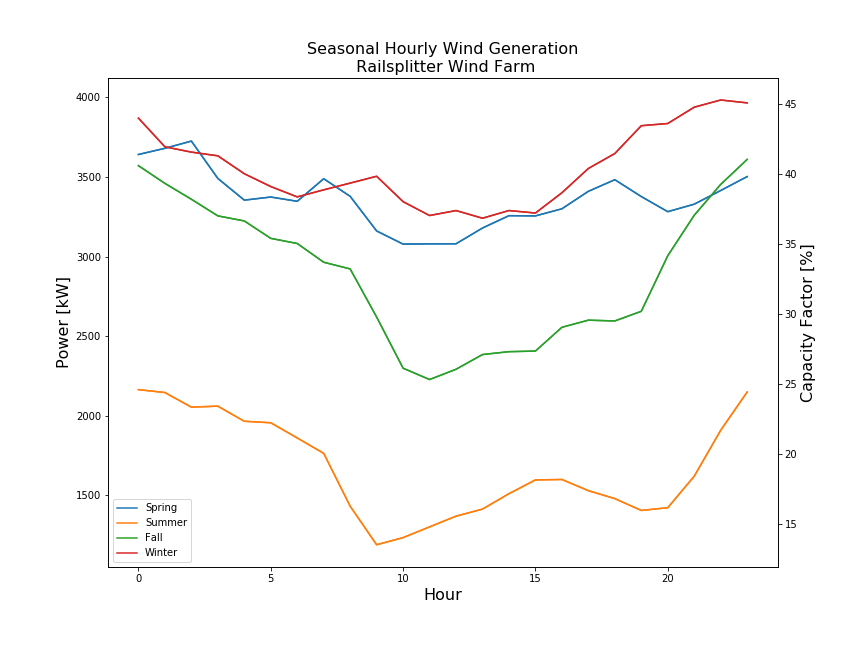
\includegraphics[width=\columnwidth]{./img/cap/seasonal_hourly_wind.png}
	\caption{<++>}
	\label{fig:<++>}
\end{figure}

\begin{figure}[ht]
	\centering
	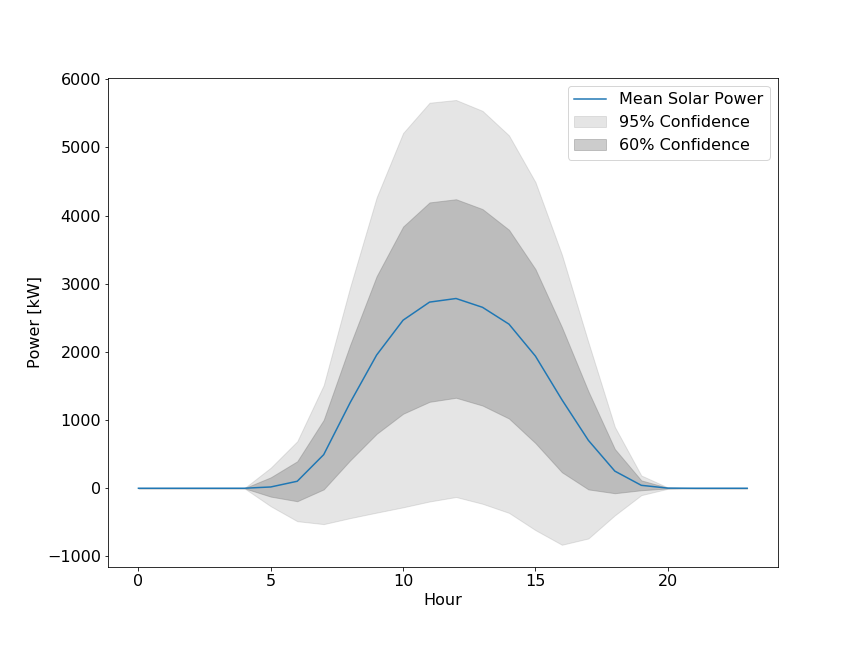
\includegraphics[width=\columnwidth]{./img/cap/solar_mean.png}
	\caption{<++>}
	\label{fig:<++>}
\end{figure}

\begin{figure}[ht]
	\centering
	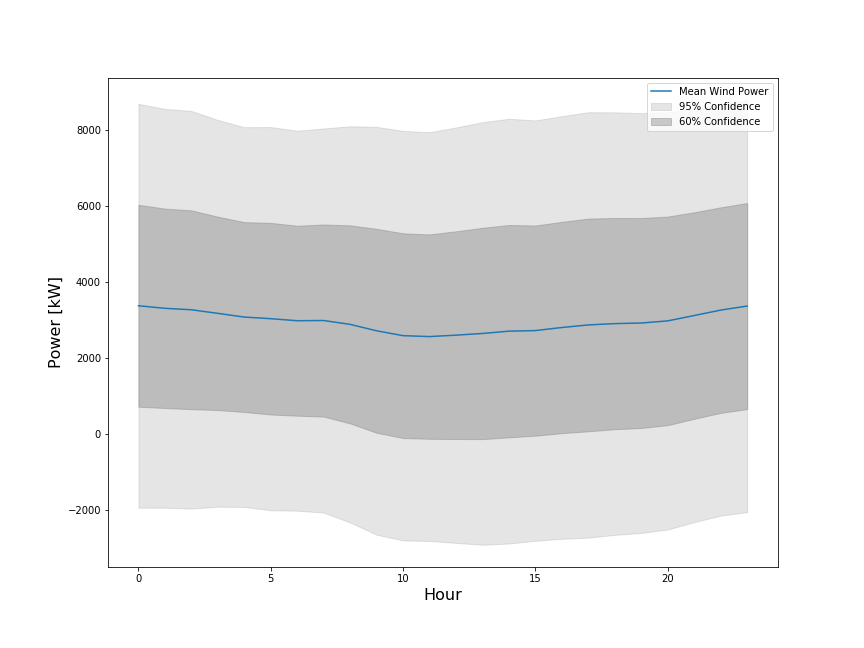
\includegraphics[width=\columnwidth]{./img/cap/wind_mean.png}
        \caption{<++>}
	\label{fig:<++>}
\end{figure}

\section{Discussion}
text

\FloatBarrier

\bibliographystyle{unsrt}
\bibliography{2021-04-nm-illinois}
\end{document}
